\section{Stand der Forschung}

Vertraulichkeit ist das erste Voraussetzung, das ein System erfüllt muss, um  potenziellen neue 
Kunden zu gewinnen. Unter diesem Begriff soll ein System nur auf autorisierte Informationen 
zugreifen \cite{refbook:SWIS}. In dieser Hinsicht soll die Entwicklung einer Click and Buy Maschine 
so konzipiert werden, damit sie einen sicheren Umgang mit den Kundendaten anbietet.


Solche Maschine kann als Cyber-Physical System klazifiziert werden \cite{inbook:MHNS}, weil sie 
eine Interaktion zwischen Nutzer und ein oder mehrere Systemen darstellt. In dieser Zusammenarbeit
spielt den Datenaustausch eine wesentliche Rolle, besonders von der Seite der Nutzender. 
Diese Technologie zielt eine günstigere Entwicklung, ohne auf die Sicherheit zu vernachlässigen.
\textbf{ich habe keine Ahnung, wie ich hier erweitern kann.}


Die zunehmende Tendenz von bargeldlose Bezahlung erfordert neuen Umgang mit der eigegebenen Daten.
Laut einer Studie von 2009 der Deutschen Bundesbank stieg rasant die Anzahl von bargeldlose Bezahlung 
in der Bundesrepublik \cite{refrep:DB}.

\begin{figure}[htb]
    \centering{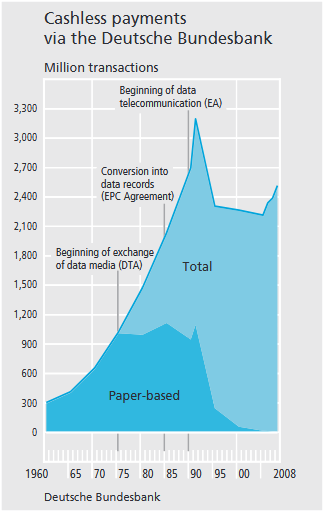
\includegraphics[width =5 cm]{Bilder/refrep_DB.png}}
    \caption{Cashless payments via the Deutsche Bundesbank}
    \label{fig:graphic}
\end{figure}

Da es sich um einen dynamischen Sektor geht, finden die Änderungen sehr schnell statt, obwohl die 
Sicherheitsmechanismen an diese Geschwindigkeit nicht immer anpassen kann \cite{refbook:MNIT}.









\textbf{Ich würde diesen Satz in den nächsten Kapitel verwenden und erweitern mit unseren Recherchen, damit wird 
die Literatur rechtfertigen können}
Um das zu bewerkstelligen, ist der aktuelle technische Stand von entscheidener Bedeutung. 
Ausgehend von dieser Informationen muss das Glasfasernetz eventuell erweitert oder auch neu verlegt werden.
Denn das Ziel ist es, technisch gesehen auf dem neusten Stand zu sein, damit das Click and Buy System für die Zukunft abgesichert ist.
Außerdem wird durch den Ausbau des Glasfasernetzes die Region insgesamt deutlich attraktiver gemacht, was vielleicht auch Menschen dazu bringt
in diese Region zu ziehen. Denn jedem ist klar, dass ein guter Internetausbau essentiell ist, um vielleicht auch mal von zuhause aus zu arbeiten.